% MICAI 2026 - Springer LNCS format
\documentclass[runningheads]{llncs}

\usepackage[utf8]{inputenc}
\usepackage[T1]{fontenc}
\usepackage{graphicx}
\usepackage{booktabs}
\usepackage{amsmath,amssymb}
\usepackage{hyperref}
\usepackage{xcolor}
\usepackage{multirow}
\usepackage{array}
\usepackage{multicol}

\hypersetup{colorlinks=true,linkcolor=blue,citecolor=blue,urlcolor=blue}

% Compactado de floats para caber en 12 páginas LNCS.
\setlength{\textfloatsep}{6pt plus 2pt minus 2pt}
\setlength{\floatsep}{6pt plus 2pt minus 2pt}
\setlength{\intextsep}{6pt plus 2pt minus 2pt}
\setlength{\abovecaptionskip}{4pt}
\setlength{\belowcaptionskip}{2pt}

% Three figures (global metrics, Sharpe boxplot, training-window effect) are
% redundant with Tables 4-5 and are shipped as supplementary material so the
% paper fits the 12-page LNCS limit. Change to \extrafigstrue to typeset them
% inline again; scripts_opt/plots_paper.py generates all of them either way.
\newif\ifextrafigs
\extrafigsfalse

\begin{document}

\title{A Benchmark of Five Machine-Learning Architectures \\for Daily Trading-Signal Classification on US Tech Equities}

\titlerunning{ML Benchmark for Daily Trading Signals}

\author{Jesus Baruc Polvo~Cuatiaquiz\inst{1} \and
Abdiel Reyes~Vera\inst{1} \and
Emmanuel Ju\'arez~Carbajal\inst{2} \and
David Reyes~Ramos\inst{1} \and
Maribel Arag\'on~Garc\'ia\inst{1}}

\authorrunning{J. B. Polvo Cuatiaquiz et al.}

\institute{Escuela Superior de C\'omputo, Instituto Polit\'ecnico Nacional, Ciudad de M\'exico, M\'exico \\
\email{barucpolvo@gmail.com}\\
\email{areyesve@ipn.mx}\\
\email{dreyesr2105@alumno.ipn.mx}\\
\email{ipnaragong@gmail.com}
\and
Centro de Investigaci\'on en Computaci\'on, Instituto Polit\'ecnico Nacional, Ciudad de M\'exico, M\'exico \\
\email{ejuarezc2023@cic.ipn.mx}}

\maketitle

\begin{abstract}
We benchmark five supervised classifiers --- multinomial logistic regression (LR), XGBoost, a bidirectional Long Short-Term Memory network (LSTM), a 1-D Convolutional Neural Network (CNN) and a hybrid CNN-LSTM --- on predicting daily BUY/HOLD/SELL signals for seven large-cap US technology stocks (AAPL, NVDA, TSLA, AMZN, MSFT, GOOGL, META). The label is the rolling 30/70-percentile of the one-day forward log-return over a 252-day window, an adaptive ground truth robust to bull and bear regimes. We use 61 indicators from daily open-high-low-close-volume (OHLCV) data plus context from the SPY exchange-traded fund (ETF) and the CBOE Volatility Index (VIX), all free from Yahoo Finance. Three temporal splits share the test year (2025) and differ only in training years (10, 6 and 4); each model is trained \emph{globally} and \emph{per ticker}, for 120 controlled runs scored on F1-macro plus win rate, profit factor and maximum drawdown. LR with elasticnet regularization attains the highest average F1-macro (0.399) and the best Sharpe in the principal experiment (+0.76), outperforming the deep architectures; re-running everything under a stricter protocol with a symmetric Optuna search and 95\,\% bootstrap intervals leaves LR significantly ahead of all four. A separate ablation shows statistical feature filtering (Pearson correlation, variance inflation factor, Spearman rank correlation and SHAP values) hurts in 11 of 15 cases: internal regularization beats external pre-selection. Finally, ticker volatility, not model class, dominates cross-asset performance variation.
\keywords{Trading signals \and Classification \and Deep learning \and Logistic regression \and XGBoost \and LSTM \and CNN.}
\end{abstract}

\section{Introduction}

Short-term equity forecasting is among the most studied problems in quantitative finance. The Efficient Market Hypothesis~\cite{fama1970} predicts no meaningful predictability; in practice, recent surveys~\cite{sezer2020,jiang2021} show machine-learning models extracting a small but exploitable signal from technical indicators. Three limitations recur: (i) comparisons involve only one or two models; (ii) the reported metric is often accuracy or root-mean-square error (RMSE), which do not translate cleanly into trading performance; (iii) univariate feature pre-selection is applied without checking it helps. This paper addresses the three jointly.

We compare five representative models --- a linear baseline (LR), a gradient-boosted tree model (XGBoost) and three deep-learning architectures (LSTM, CNN, CNN-LSTM) --- under an identical protocol across 120 controlled runs (5 models $\times$ 3 splits $\times$ 8 modalities). All runs share the same test year (2025); only the amount of training history differs (10, 6 or 4 years). Every run reports F1-macro together with win rate, profit factor and maximum drawdown.

\paragraph{Contributions.}
(i) a reproducible pipeline on free Yahoo Finance data, with temporally aligned
splits that isolate training-window size; (ii) a five-model benchmark of 120 runs
under one protocol, evaluated both as classification and as economics; (iii) an
empirical assessment of statistical feature pre-selection (Pearson, VIF, Spearman,
SHAP) against simply keeping every feature; (iv) evidence that ticker volatility,
not model choice, explains most of the cross-asset variance in Sharpe; and (v) a
re-run of the whole comparison under a stricter protocol with a symmetric
hyper-parameter search and bootstrap confidence intervals.

\section{Related Work}
\label{sec:related}

Sezer et al.~\cite{sezer2020} review more than 140 papers on deep learning for financial time series and observe that LSTM and CNN dominate the published architectures while linear baselines are rarely included. Fischer and Krauss~\cite{fischer2018} apply LSTM to S\&P 500 constituents and report positive abnormal returns, although later replications raise look-ahead concerns in the percentile-based label. Patel et al.~\cite{patel2015} compare support vector machines (SVM), artificial neural networks (ANN) and random forests on the Indian market and find well-regularized linear and tree models matching deep networks at daily horizons. XGBoost~\cite{chen2016} remains the strong tree baseline; we tune it with the Tree-structured Parzen Estimator (TPE) sampler of Optuna~\cite{akiba2019}. We are not aware of a side-by-side comparison of LR, XGBoost and three deep architectures under one protocol with both classification and economic evaluation; that is the gap addressed here.

\section{Data and Target}
\label{sec:data}

\subsection{Assets and source}

We use the seven largest US technology stocks by market capitalization at the end of 2024: AAPL, NVDA, TSLA, AMZN, MSFT, GOOGL and META. Daily OHLCV data from 2013-12-31 to 2025-12-29 are downloaded with the \texttt{yfinance} library, with adjustments for splits and dividends. Market context is added through SPY (the S\&P 500 ETF) and \verb|^|VIX. No paid data source is used; the entire pipeline runs on freely available Yahoo Finance data.

\subsection{Target construction}

Let $C_t$ be the close price on day $t$. The forward log-return is
\begin{equation}
r_{\text{fwd}}(t) = \ln\frac{C_{t+1}}{C_t}.
\end{equation}
Over a rolling window of $W = 252$ trading days, we compute the 30th and 70th percentiles of $r_{\text{fwd}}$ using only data available before day $t$. The label is
\begin{equation}
y_t = \begin{cases}
\mathrm{BUY}\;(2) & \text{if } r_{\text{fwd}}(t) \ge q_{70}(t-1),\\
\mathrm{SELL}\;(0) & \text{if } r_{\text{fwd}}(t) \le q_{30}(t-1),\\
\mathrm{HOLD}\;(1) & \text{otherwise.}
\end{cases}
\end{equation}
By construction the class distribution is close to 30/40/30 in every market regime, removing the need to set an arbitrary $\alpha\sigma$ threshold. The shift by one day in the quantile computation prevents look-ahead.

\subsection{Features (61 in total)}

We compute the indicators in Table~\ref{tab:features}. All values are derived from daily OHLCV plus SPY and VIX. Seasonality variables are encoded as sine/cosine pairs to preserve periodicity. No fundamentals, news or option data are used. The abbreviations in the table are the standard ones: MA (moving average), ATR (average true range), RSI (relative strength index), MACD (moving-average convergence/divergence), Stoch (stochastic oscillator), OBV (on-balance volume), VWAP (volume-weighted average price), CMF (Chaikin money flow) and MFI (money flow index).

The 61 features span nine families: log returns (5: ret\_$\{1,2,3,5,10\}$d),
momentum (4: mom\_$\{5,10,20,60\}$d), moving-average distances and crossovers
(9), volatility (8: ATR(14), realized vol 5/10/20/60d, ratios), oscillators (9:
RSI(7,14), MACD/signal/histogram, stochastic K/D/diff, Williams \%R), volume and
flow (8: OBV, VWAP distance, CMF(20), MFI(14), volume ratios), candle patterns
(7), seasonality (5: weekday and month as sine/cosine pairs, week-of-month) and
market context (6: SPY return, 20-day volatility and momentum; VIX level, change
and normalized).

\subsection{Temporal splits}

We define three splits that share the same out-of-sample year (2025) and only differ in the amount of training history (Table~\ref{tab:splits}). This design isolates the effect of training-window length, at the cost of a single market regime (Section~\ref{sec:limitations}).

\begin{table}[t]
\centering
\caption{Temporal splits. All three share the same test year (2025) for direct comparison.}
\label{tab:splits}
\begin{tabular}{ccccc}
\toprule
Experiment & Train & Validation & Test & Train years \\
\midrule
A & 2014--2023 & 2024 & 2025 & 10 \\
B & 2018--2023 & 2024 & 2025 & 6 \\
C & 2020--2023 & 2024 & 2025 & 4 \\
\bottomrule
\end{tabular}
\end{table}

\paragraph{Is 2025 a representative test year?}
Averaged over the seven tickers, 2025 returned $+24.2\,\%$ (2014--2024 median
$+46.3\,\%$, 9th of twelve), with realized volatility $39.1\,\%$ (3rd highest),
mean maximum drawdown $-33.0\,\%$ and mean VIX 19.0; label balance was
29.6/42.2/28.3 against 30.0/40.0/30.0 over 2014--2025. All four market
statistics fall inside the 2014--2024 range, but the year is below-median on
return and above-median on volatility --- not the easy bull market that would
flatter a long-biased classifier. That makes 2025 defensible as a single
choice, not a substitute for multiple test years (Section~\ref{sec:limitations}).

\section{Models}
\label{sec:models}

\paragraph{Logistic regression (LR).}
A multinomial logistic regressor with elasticnet penalty~\cite{zou2005} ($\ell_1+\ell_2$, SAGA solver). The grid over $C \in \{0.01, 0.1, 1\}$ and $l_1\text{-ratio}=0.5$ is searched on validation; class weights are balanced; multi-seed averaging combines five seeds by majority vote.

\paragraph{XGBoost.}
Gradient-boosted trees with \texttt{multi:softprob} objective and \texttt{hist} method on GPU. Hyper-parameters are tuned with Optuna~\cite{akiba2019} (TPE sampler) for 20 to 40 trials per setting, targeting validation F1-macro. Sample weights are balanced; three random seeds are averaged by soft-voting.

\paragraph{LSTM (bidirectional).}
Two stacked bidirectional LSTM~\cite{hochreiter1997} layers (hidden=128, dropout=0.3) followed by layer normalization and a linear head. We evaluate look-back windows of 20 and 60 trading days. The last hidden state feeds the classifier. Three seeds are averaged.

\paragraph{1-D CNN.}
Three Conv1D~\cite{lecun1989} blocks (filters 64-128-192, kernel=3, batch normalization (BN), ReLU activation, dropout) followed by global average $+$ max pooling along the temporal axis. Two dense layers produce the logits. No recurrence is used.

\paragraph{CNN-LSTM.}
A CNN front-end (filters 64-128) extracts local patterns; its output is fed into an LSTM (hidden=128, two layers) that captures longer dependencies. A linear head produces the logits. The last five input channels carry locally normalized OHLCV (each window divided by its first close and max volume) so that the CNN learns scale-invariant candle shapes.

\paragraph{Training and selection.}
Scalers are fitted inside each split (\texttt{StandardScaler} for LR, \texttt{MinMaxScaler} for the deep models; XGBoost takes raw values). The deep models train for up to 80 epochs with AdamW, gradient clipping at 1.0, \texttt{ReduceLROnPlateau} and early stopping with patience 15 on validation loss --- a criterion Section~\ref{sec:robust} shows to be the binding one. Each run's prediction averages three random-seed checkpoints (five for LR).

\section{Evaluation}
\label{sec:eval}

\subsection{Classification}
We use \textbf{F1-macro} as the primary metric: the unweighted mean of the per-class F1 scores. Macro averaging gives equal weight to the BUY, HOLD and SELL classes, which is appropriate given the deliberate near-balance of the label distribution. Per-class F1 for every run is included in the supplementary material.

\subsection{Backtest}
For every test day the predicted label is mapped to a position (BUY $\to$ +1, HOLD $\to$ 0, SELL $\to$ $-1$) and the daily strategy return is $r_{\text{strat}}(t) = \text{position}(t)\cdot r_{\text{fwd}}(t)$. Over the days on which the model takes a position (HOLD excluded) we report the \textbf{win rate}, the fraction with $r_{\text{strat}} > 0$, and the \textbf{profit factor} $\sum r_{\text{strat}}^{+} / |\sum r_{\text{strat}}^{-}|$; over the cumulative equity curve we report the \textbf{maximum drawdown}, $\min (\text{equity}_t - \text{peak}_t)/\text{peak}_t$, and the \textbf{annualized Sharpe ratio} $\sqrt{252}\,\bar r_{\text{strat}}/\sigma_{r_{\text{strat}}}$ with $r_f = 0$. Transaction costs and slippage are deliberately omitted: the aim is a first-order comparison between models under identical conditions.

\subsection{A note on accuracy}
We do not report accuracy. With three near-equally-distributed classes, the classifier can reach $\approx$~0.40 accuracy by predicting only HOLD, which is uninformative. F1-macro penalizes such collapse.

\section{Statistical feature pre-selection: should we use it?}
\label{sec:featselect}

A common preliminary step is to filter features by statistical test: Pearson correlation against the target and the Variance Inflation Factor (VIF) for multicollinearity (suited to LR), SHapley Additive exPlanations (SHAP)~\cite{lundberg2017} rank (suited to tree models), or Spearman rank correlation (for the non-linear models). On the same code path we compared every model trained on all 61 features against the same model trained only on the features that passed its test on validation.

\begin{table}[t]
\centering
\caption{Effect of statistical pre-selection on GLOBAL F1-macro: $\Delta = \text{F1}(\text{all 61}) - \text{F1}(\text{filtered})$. A positive value means that using all features is better.}
\label{tab:featselect}
\begin{tabular}{llccc}
\toprule
Model & Filter & Exp A & Exp B & Exp C \\
\midrule
LR & Pearson + VIF (4--8 feats)& $+0.024$ & $+0.026$ & $+0.021$ \\
XGBoost & SHAP top-$N$ (23--25 feats)& $+0.009$ & $+0.021$ & $+0.022$ \\
LSTM & Spearman (3--25 feats)& $+0.039$ & $+0.036$ & $-0.006$ \\
CNN 1D & Spearman & $+0.035$ & $-0.025$ & $+0.011$ \\
CNN-LSTM & Spearman & $-0.011$ & $+0.020$ & $-0.026$ \\
\bottomrule
\end{tabular}
\end{table}

\paragraph{Result and decision.}
Table~\ref{tab:featselect} shows that in 11 of 15 cases keeping all 61 features beats the filtered subset. The deltas are largest for LR, the model with the strongest internal regularization, where the elasticnet penalty performs implicit selection more effectively than an external Pearson/VIF screen; for XGBoost the SHAP filter is competitive, as expected for a tree model; for the deep models the sign depends on the experiment. All subsequent results therefore use the full 61 features for every model. These tests remain useful as exploratory tools --- to report which indicators dominate --- but not as a pre-training filter.

\section{Results}
\label{sec:results}

We report 120 controlled runs (5 models $\times$ 3 splits $\times$ (1 global + 7 per-ticker)). For the sequence models (LSTM, CNN, CNN-LSTM) we trained look-backs of 20 and 60 days and report the better of the two \emph{as measured on the test set}; this deliberately generous choice gives the deep models an oracle advantage that LR and XGBoost do not get, so the gaps below are a lower bound on LR's margin. Section~\ref{sec:robust} repeats the comparison with no test-set information used for selection.

\subsection{Global models}

Table~\ref{tab:f1_global} shows F1-macro on the 2025 test set when one single model is trained on the concatenated data of all seven tickers. LR leads on average (0.399) and wins two of the three experiments outright. XGBoost is the runner-up and edges LR by 0.002 in Exp B. The deep models cluster lower, around 0.34--0.39.

\begin{table}[t]
\centering
\caption{F1-macro on the 2025 test set, GLOBAL strategy. Best per column in bold.}
\label{tab:f1_global}
\begin{tabular}{lcccc}
\toprule
Model & Exp A (10y) & Exp B (6y) & Exp C (4y) & Avg \\
\midrule
LR & \textbf{0.411} & 0.385 & \textbf{0.401} & \textbf{0.399} \\
XGBoost & 0.396 & \textbf{0.386} & 0.373 & 0.385 \\
LSTM & 0.389 & 0.370 & 0.370 & 0.376 \\
CNN-LSTM & 0.376 & 0.384 & 0.371 & 0.377 \\
CNN 1D & 0.361 & 0.343 & 0.373 & 0.359 \\
\midrule
Random 1/3 & 0.333 & 0.333 & 0.333 & 0.333 \\
\bottomrule
\end{tabular}
\end{table}

\ifextrafigs
\begin{figure}[t]
\centering
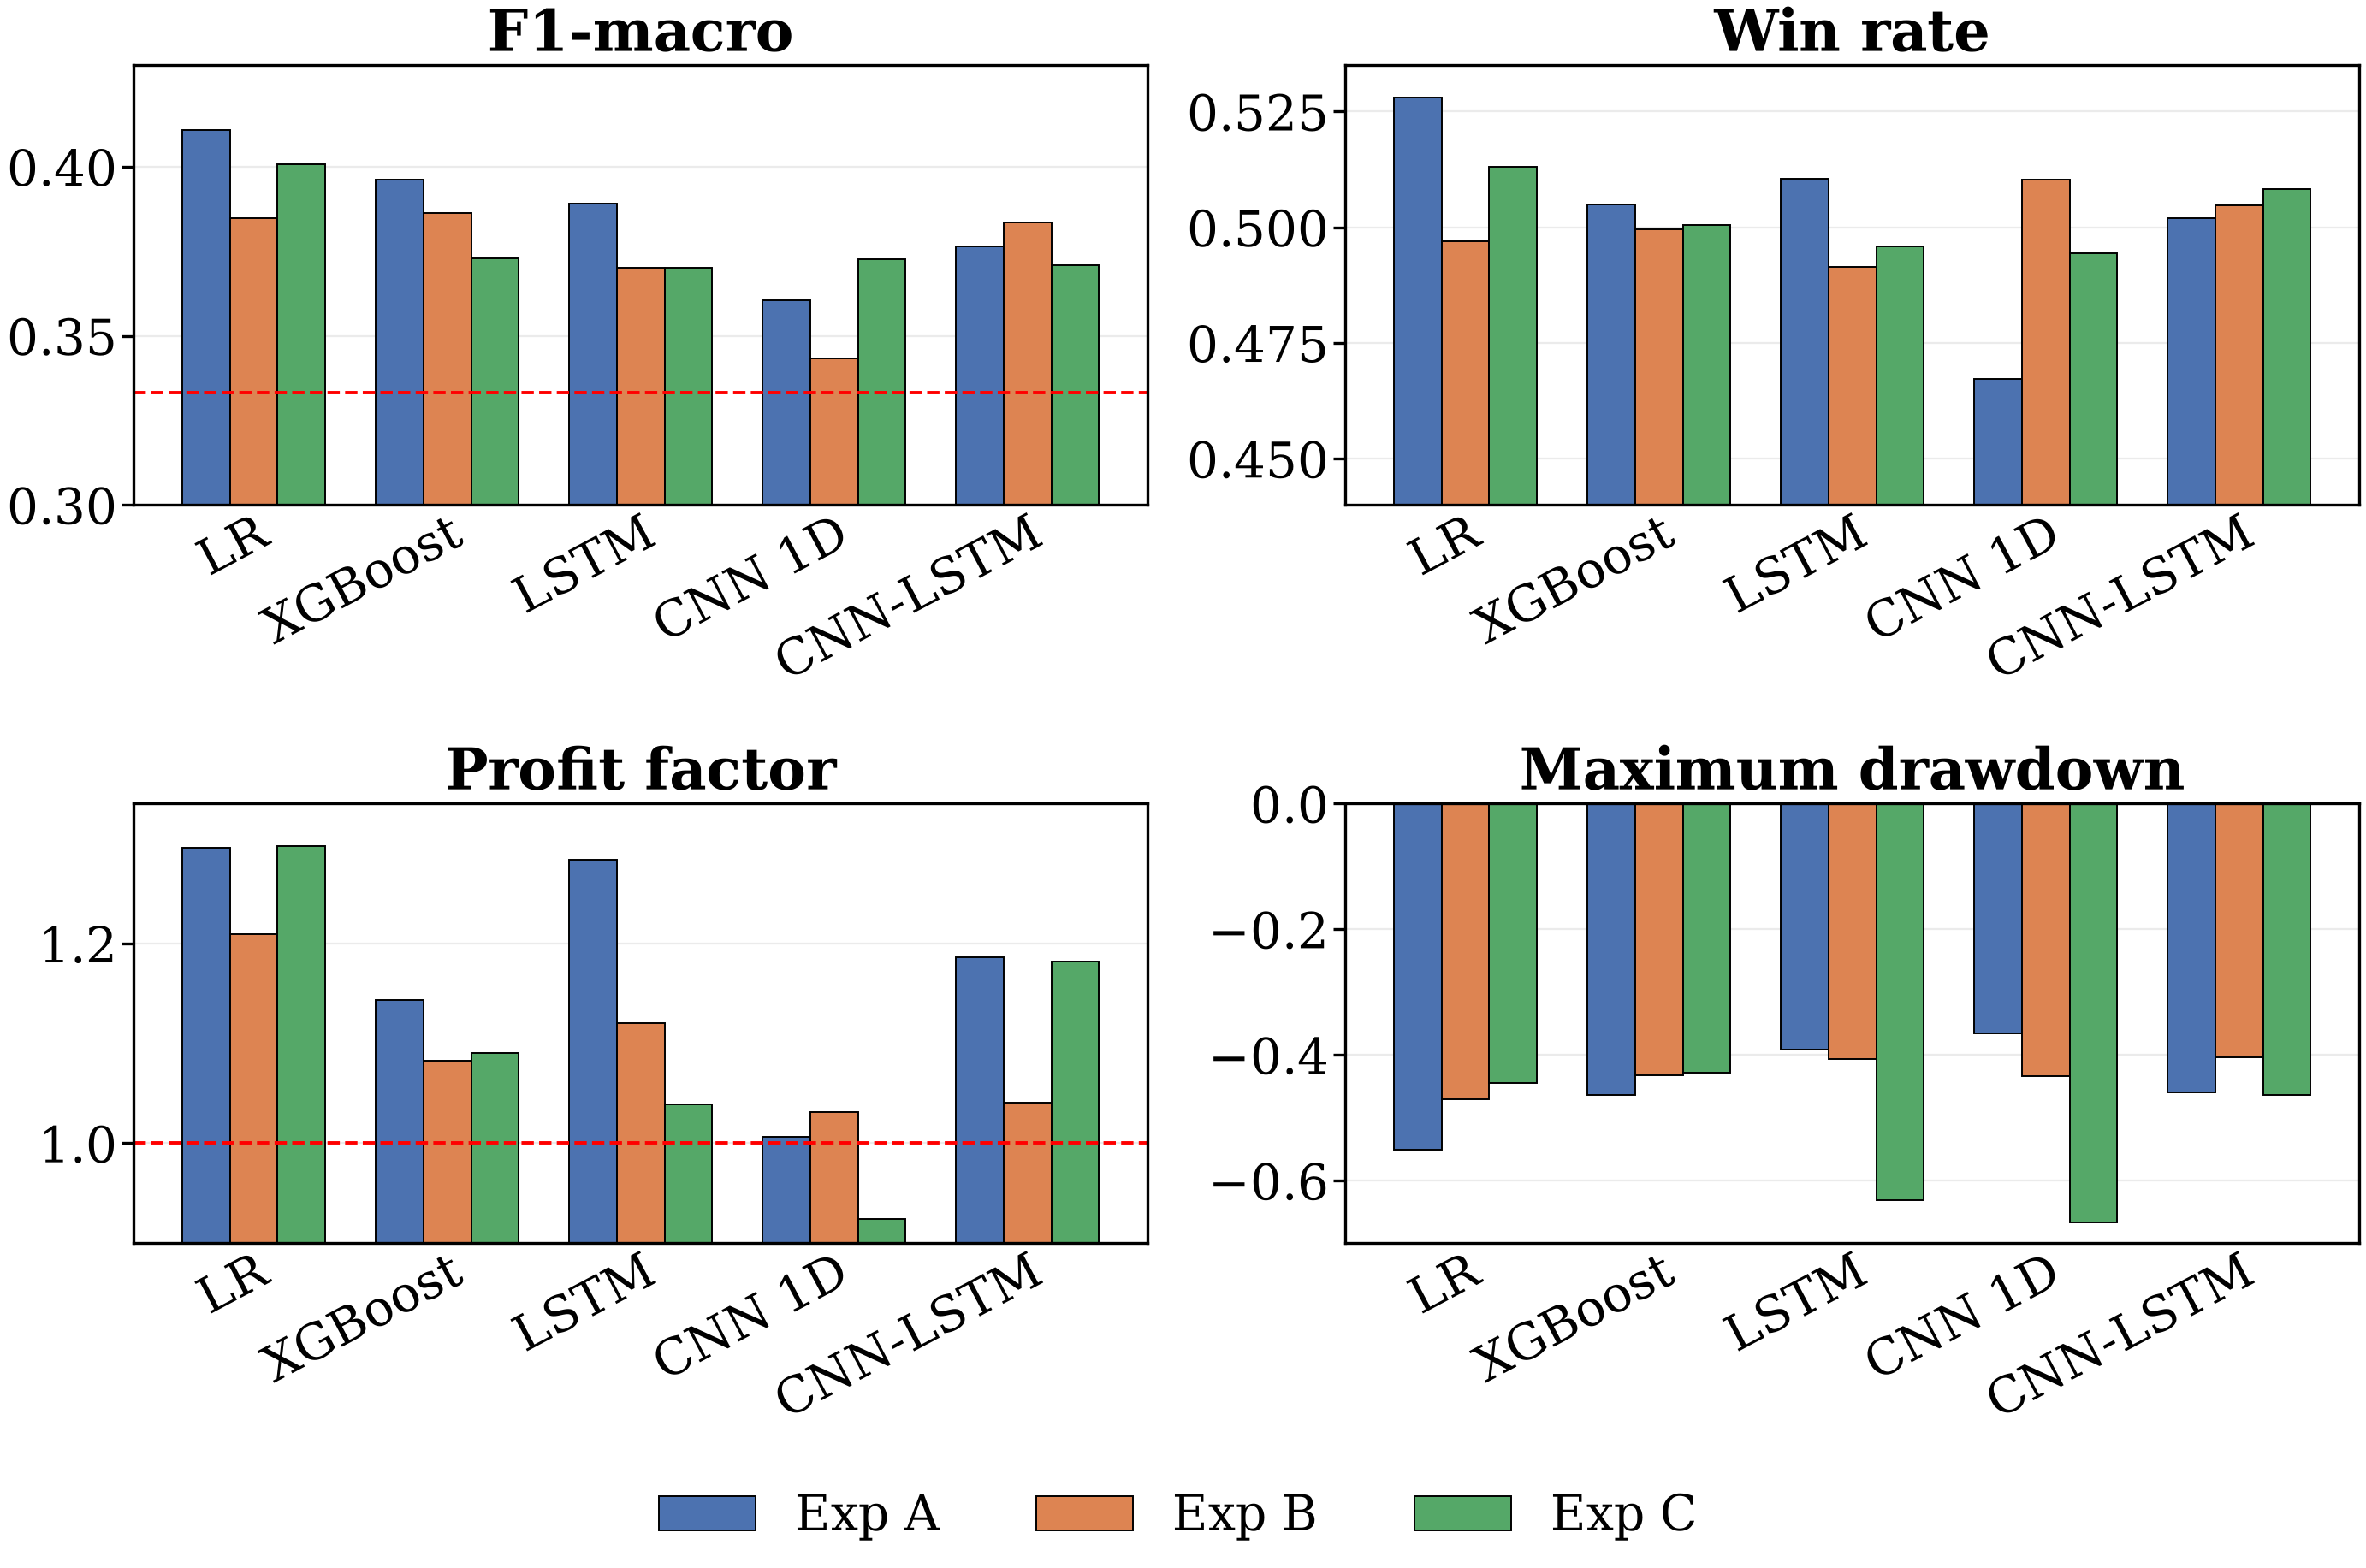
\includegraphics[width=\textwidth]{figures/fig_global_metrics.png}
\caption{Global models on the 2025 test set: F1-macro (top-left), win rate (top-right), profit factor (bottom-left) and maximum drawdown (bottom-right). The dashed red line in the F1 panel marks the 1/3 random baseline. Higher is better except for drawdown.}
\label{fig:global}
\end{figure}
\fi

The economic metrics tell a more nuanced story (Table~\ref{tab:econ_B}). For the recommended experiment (Exp B), LR has the highest profit factor (1.21) and Sharpe (+0.76). XGBoost matches the F1 but its strategy is closer to random in economic terms. CNN-LSTM controls drawdown best ($-0.40$). The pure CNN is the weakest both in F1 and Sharpe. The same four metrics for Exps A and C are in the supplementary material.

\begin{table}[t]
\centering
\small
\caption{Economic metrics on Exp B GLOBAL (test = 2025). Sharpe is annualized.}
\label{tab:econ_B}
\begin{tabular}{lccccc}
\toprule
Model & F1 & Win rate & Profit factor & Max drawdown & Sharpe \\
\midrule
LR & 0.385 & 0.497 & \textbf{1.210} & $-0.470$ & \textbf{+0.755} \\
XGBoost & \textbf{0.386} & 0.500 & 1.083 & $-0.432$ & +0.345 \\
CNN-LSTM & 0.384 & \textbf{0.505} & 1.041 & \textbf{$-0.403$} & +0.147 \\
LSTM & 0.370 & 0.491 & 1.120 & $-0.406$ & +0.433 \\
CNN 1D & 0.343 & 0.510 & 1.031 & $-0.434$ & +0.121 \\
\bottomrule
\end{tabular}
\end{table}

\subsection{Per-ticker models}

When one model is trained per ticker (Table~\ref{tab:f1_pt}), LR is again the most consistent: it leads in all three experiments. The deep models drop more visibly compared to the global setting, because each per-ticker training set contains only $\sim$1500 samples. XGBoost remains a solid second.

\begin{table}[t]
\centering
\caption{Average F1-macro across 7 tickers, PER-TICKER strategy. Best per column in bold.}
\label{tab:f1_pt}
\begin{tabular}{lcccc}
\toprule
Model & Exp A & Exp B & Exp C & Avg \\
\midrule
LR & \textbf{0.411} & \textbf{0.392} & \textbf{0.359} & \textbf{0.387} \\
XGBoost & 0.376 & 0.370 & 0.352 & 0.366 \\
CNN-LSTM & 0.368 & 0.342 & 0.356 & 0.355 \\
LSTM & 0.314 & 0.353 & 0.326 & 0.331 \\
CNN 1D & 0.378 & 0.332 & 0.280 & 0.330 \\
\bottomrule
\end{tabular}
\end{table}

\subsection{Where does the cross-asset variation come from?}
\label{sec:crossasset}

Figure~\ref{fig:sharpe_heatmap} breaks down the annualized Sharpe by model and ticker. Horizontal bands are visible: AMZN is green across almost every model, while GOOGL is mostly red. This is a property of the assets, not of the models: the more directionally tradeable tickers (high realized volatility, well-defined trends) reward any reasonable classifier, while range-bound tickers punish all of them. Decomposing the total sum of squares of the 105 per-ticker Sharpe values confirms it: the ticker accounts for 15.5\,\% of the variation and the model for only 3.4\,\% (the experiment adds 7.0\,\%, and 74.1\,\% is interaction and run-to-run noise). The ticker therefore explains roughly $4.5\times$ as much Sharpe variation as the choice of model.

\begin{figure}[t]
\centering

\includegraphics[width=0.85\textwidth]{figures/fig_sharpe_heatmap.png}
\caption{Annualized Sharpe ratio per model and ticker, for the three experiments (test = 2025).}
\label{fig:sharpe_heatmap}
\end{figure}

Collapsed over models, the interquartile range of a single ticker spans more
Sharpe than the gap between the best and worst model class: AMZN leads on both
mean and median, GOOGL is the only ticker with a negative mean ($-0.15$) and NVDA
the only one with a negative median ($-0.16$) despite a positive mean.

\ifextrafigs
\begin{figure}[t]
\centering

\includegraphics[width=0.85\textwidth]{figures/fig_sharpe_boxplot.png}
\caption{Sharpe distribution per ticker over the 15 (model, experiment) combinations, ordered by median. Diamonds mark the mean.}
\label{fig:sharpe_box}
\end{figure}
\fi

\subsection{Effect of the training-window length}

The three splits share the same test year, so any difference between them is purely the effect of how many years of history the model can fit. In Table~\ref{tab:f1_global} LR does best with the longest history (Exp A, 10 years: 0.411), but the relation is not monotone: the 4-year window (Exp C: 0.401) recovers most of that and beats the 6-year window (Exp B: 0.385). The deep models are largely flat across the three windows, indicating that more history does not help much when capacity is fixed and the optimizer is the bottleneck. With a single test year the spread between windows (0.026 for LR) is of the same order as the run-to-run noise reported in Section~\ref{sec:robust}, so we do not read a trend into it.

\ifextrafigs
\begin{figure}[t]
\centering

\includegraphics[width=\textwidth]{figures/fig_train_years.png}
\caption{Effect of training-window length on F1-macro (left) and Sharpe (right). All settings test on year 2025.}
\label{fig:trainyears}
\end{figure}
\fi

\subsection{Signal distribution}

Figure~\ref{fig:signaldist} shows the predicted BUY/HOLD/SELL distribution for the five global models on Exp B. The realized base rate is 30.0/40.0/30.0 over 2014--2025 and 29.6/42.2/28.3 in the test year, so the label construction of Section~\ref{sec:data} behaves as intended. The CNN is the outlier: it collapses towards BUY (49\,\%) and almost abandons SELL (6\,\%), consistent with its lowest F1. LSTM and XGBoost track the prior most closely, while LR is conservative on BUY (18\,\%) and long on SELL (38\,\%) --- which is what earns it the best Sharpe in a test year whose mean return was below the historical median. A predicted distribution far from the prior is thus a useful diagnostic of over-confidence or of a degenerate solution.

\begin{figure}[t]
\centering

\includegraphics[width=0.85\textwidth]{figures/fig_signal_dist.png}
\caption{Predicted distribution of the three signals for the global models on Exp B (test=2025). Dotted lines indicate the 33.3\,\% / 66.6\,\% references.}
\label{fig:signaldist}
\end{figure}

\subsection{Drill-down on the best model per ticker}
\label{sec:drilldown}

For the seven per-ticker XGBoost models of Exp B (highest global F1), TSLA is the outlier --- F1 0.44, Sharpe $+2.06$, +201\,\% cumulative return, 60\,\% win rate, drawdown $-0.20$ --- and GOOGL is the worst, F1 0.34, Sharpe $-0.88$, cumulative $-21\,\%$. NVDA reaches Sharpe $+1.41$ despite an F1 of 0.34; AMZN, MSFT, META and AAPL cluster in F1 $\in [0.34, 0.40]$ with Sharpes between $-0.06$ and $+0.71$. The best-to-worst spread (0.44 vs.\ 0.34 in F1, $+2.06$ vs.\ $-0.88$ in Sharpe) is far wider than the spread across model classes in Table~\ref{tab:f1_global}.

\section{Robustness: symmetric search and confidence intervals}
\label{sec:robust}

Two asymmetries in Section~\ref{sec:results} could by themselves explain the ranking: XGBoost was tuned by Optuna while the deep models got only a small hand-built grid over \texttt{hidden}, \texttt{layers} and \texttt{dropout} --- without the learning rate or the weight decay --- and their look-back was picked on the test set. We re-ran the whole comparison under a protocol that removes both.

\paragraph{Protocol.}
Three roles are separated. In \emph{dev} mode the models train on 2018--2022, the
epoch checkpoint is selected on 2023, and every configuration decision --- ablations
and the hyper-parameter search --- is taken on 2024. In \emph{final} mode they train
on 2018--2023, the checkpoint is selected on 2024, and 2025 is evaluated exactly
once per frozen configuration, so no test-set quantity enters any decision. Input
windows are also built over the continuous series and assigned to a split by the
date of the label, so all five models are scored on the same 1\,736 test rows;
previously the sequence models saw 1\,596 rows at look-back 20 and 1\,316 at 60,
which made the columns of Table~\ref{tab:f1_global} not strictly comparable.
Reproducing the published pipeline inside the new code gives identical numbers in
18 of 18 cells, so what follows is the protocol, not the reimplementation.

\paragraph{Search budget.}
Every model is now tuned by the same Optuna TPE sampler on the same decision year (Table~\ref{tab:robust}). The deep models search 17--20 hyper-parameters --- learning rate, weight decay, cross-entropy vs.\ focal loss, label smoothing, temporal pooling, scaler and look-back --- against the 9 of XGBoost and the 5 of LR; of 80 trials each, 54/53/74 (LSTM/CNN/CNN-LSTM) completed and the rest were pruned. One full deep training takes 7--12\,s on a consumer GPU, so the binding constraint is statistical power, not compute.

\begin{table}[t]
\centering
\small
\caption{Exp B GLOBAL under the corrected protocol (test = 2025). \emph{Trials} and
\emph{H-par} are the search budget, spent entirely on the 2024 decision year; CI is
a 95\,\% block bootstrap; $\Delta$ is the F1 change from Table~\ref{tab:econ_B}.}
\label{tab:robust}
\begin{tabular}{lcccccc}
\toprule
Model & Trials & H-par & F1-macro & 95\,\% CI & $\Delta$ & Sharpe \\
\midrule
LR & 150 & 5 & \textbf{0.404} & [0.379, 0.428] & $+0.019$ & \textbf{+0.895} \\
CNN-LSTM & 80 & 19 & 0.372 & [0.346, 0.395] & $-0.011$ & $-0.074$ \\
LSTM & 80 & 17 & 0.369 & [0.341, 0.395] & $-0.001$ & $-0.345$ \\
XGBoost & 150 & 9 & 0.359 & [0.334, 0.381] & $-0.027$ & +0.462 \\
CNN 1D & 80 & 20 & 0.359 & [0.332, 0.386] & $+0.016$ & $-0.459$ \\
\bottomrule
\end{tabular}
\end{table}

\paragraph{Result.}
A serious search does \emph{not} close the gap: in Table~\ref{tab:robust} LR stays
first and its margin grows. On the bootstrap intervals LR is significantly better
than all four others (paired differences $+0.045$ over XGBoost, $+0.035$ over LSTM,
$+0.031$ over CNN-LSTM, $+0.045$ over CNN 1D, all excluding zero), while none of the
six differences \emph{among} the other four is significant. Averaged over the three
splits LR gains $+0.005$ against Section~\ref{sec:results}, XGBoost loses $0.025$,
and the two weakest deep models lose most (CNN $-0.054$, CNN-LSTM $-0.059$) ---
consistent with the test-set look-back of Section~\ref{sec:results} having
flattered them. The economic separation is wider still: all three deep models fall
to a profit factor below 1 and a negative Sharpe once that oracle is removed, while
LR reaches $+0.895$ at a profit factor of 1.27.

\paragraph{What actually moved the deep models.}
The largest lever was not a hyper-parameter: selecting the checkpoint by validation
F1 rather than validation loss is worth $+0.059$ F1 to the LSTM, more than the
entire spread among the deep models in Table~\ref{tab:f1_global} --- under the old
criterion validation loss rose almost monotonically from epoch 1, so the restored
checkpoint was effectively the first or second. Two further diagnostics bound what
tuning can achieve: validation loss never falls appreciably below $\ln 3 = 1.0986$
in any configuration, and shrinking the LSTM from 592\,k to 10\,k parameters
changes nothing --- the limit is neither capacity nor regularization. Retraining on
train\,$+$\,validation, which only LR and XGBoost did, makes all three deep models
\emph{worse} ($-0.024$ to $-0.047$).

\section{Discussion}
\label{sec:discussion}

\paragraph{Why does LR win on F1?}
With approximately 1500 training samples per ticker (10\,500 globally) and 61 inputs, deep models with $10^5$--$10^6$ parameters are firmly in an overfitting regime. The technical indicators already capture most of the linear predictive content of price action; the elasticnet penalty selects an effective subset of them automatically and stabilizes the remaining coefficients. XGBoost shows similar resilience because tree pruning and the $\ell_2$ leaf penalty play the same role. This matches a broader finding: on tabular data with engineered features, tree-based and linear models often match or beat deep networks~\cite{grinsztajn2022}. The asset-pricing literature is instructive about \emph{when} that ordering flips: Gu et al.~\cite{gukellyxiu2020} rank neural networks first, but on $\sim$30\,000 stocks over 60 years and for a continuous target rather than a three-way daily sign; Fischer and Krauss~\cite{fischer2018} report LSTM gains on the full S\&P 500 rather than seven tickers, while Patel et al.~\cite{patel2015} reach our conclusion at a comparable sample size. Our result locates the regime where deep learning does not pay --- short daily histories, a near-noise one-day label, features that are already multi-day aggregates --- and Section~\ref{sec:robust} shows a serious search does not rescue it.

\paragraph{Why is the cross-asset variation so large?}
Section~\ref{sec:crossasset} indicates that the model accounts for a smaller share of Sharpe variance than the ticker does. Tickers with persistent trends or high realized volatility (AMZN, TSLA, NVDA) reward any reasonably calibrated classifier; range-bound tickers (GOOGL) do not. This has practical consequences: a portfolio constructor would do better to pre-screen tickers by predictability than to choose a more elaborate model class.

\paragraph{Pooling and when to use deep models.}
Pooling all tickers helps XGBoost in all three experiments and the deep models in seven of nine (Tables~\ref{tab:f1_global} and~\ref{tab:f1_pt}) --- expected when it multiplies the sample by seven --- but is a wash for LR, which already regularizes hardest. As for the deep models themselves: under Section~\ref{sec:results}'s protocol the LSTM and CNN-LSTM contain drawdown better than LR ($-0.41$ and $-0.40$ vs.\ $-0.47$), but that advantage vanishes under Section~\ref{sec:robust} ($-0.68$ and $-0.62$). They become attractive with longer histories or richer inputs; neither condition is met here.

\section{Limitations}
\label{sec:limitations}

We do not include transaction costs or slippage; under realistic costs the rank order between models with $\text{Sharpe}\!<\!0.5$ would likely flip toward the strategy that trades least. The sample is restricted to seven large-cap US tech stocks, so conclusions need not generalize to other sectors or markets. Position sizing is binary ($\pm 1$ or $0$); a Kelly or volatility-targeted scheme would change absolute Sharpe figures while keeping the relative ranking. We use a single split per experiment; walk-forward, purged cross-validation~\cite{lopezdeprado2018} would tighten confidence intervals at higher compute cost.

The main limitation is that all three splits test on 2025. Section~\ref{sec:data} argues the year is not anomalous and Section~\ref{sec:robust} attaches bootstrap intervals, but a single period cannot fully separate a model effect from a year-specific regime; rolling the protocol over several test years remains the most valuable extension. Two caveats: our search is symmetric in \emph{procedure} but not in \emph{dimension} (80 trials over 17--20 deep hyper-parameters vs.\ 150 over XGBoost's 9), so we claim only that a realistic search does not overturn the ranking; and the conclusion is scoped to this representation, where multi-day aggregates over a short window are close to the worst case for a sequence model.

\section{Conclusions}
\label{sec:conclusions}

A multinomial logistic regression with elasticnet regularization, trained on 61 indicator features from free Yahoo Finance data, beats three deep architectures and a tuned XGBoost on average F1-macro across three temporal splits and matches or exceeds them economically --- and its margin survives a symmetric hyper-parameter search, a selection protocol that touches no test data, and bootstrap confidence intervals. Statistical feature pre-selection does not help: keeping all features and relying on the model's own regularization wins in 11 of 15 cases. Ticker volatility, not model class, explains the bulk of the cross-asset Sharpe variation. For daily large-cap data with no alternative datasets, a well-regularized linear classifier is a competitive and cheap default; deep models become attractive only with longer histories or richer inputs. All code, data manifests, fixed random seeds and library versions are available in the supplementary material.

{\footnotesize
\setlength{\columnsep}{12pt}
\begin{multicols}{2}
\begin{thebibliography}{99}
\setlength{\itemsep}{0.5pt plus 0.5pt minus 0.5pt}
\setlength{\parskip}{0pt}
\raggedright

\bibitem{fama1970}
Fama, E. F.: Efficient capital markets: A review of theory and empirical work. The Journal of Finance \textbf{25}(2), 383--417 (1970)

\bibitem{sezer2020}
Sezer, O. B., Gudelek, M. U., Ozbayoglu, A. M.: Financial time series forecasting with deep learning: A systematic literature review. Applied Soft Computing \textbf{90}, 106181 (2020)

\bibitem{fischer2018}
Fischer, T., Krauss, C.: Deep learning with long short-term memory networks for financial market predictions. European Journal of Operational Research \textbf{270}(2), 654--669 (2018)

\bibitem{jiang2021}
Jiang, W.: Applications of deep learning in stock market prediction: recent progress. Expert Systems with Applications \textbf{184}, 115537 (2021)

\bibitem{patel2015}
Patel, J., Shah, S., Thakkar, P., Kotecha, K.: Predicting stock and stock price index movement using trend deterministic data preparation and machine learning techniques. Expert Systems with Applications \textbf{42}(1), 259--268 (2015)

\bibitem{chen2016}
Chen, T., Guestrin, C.: XGBoost: A scalable tree boosting system. In: Proc. KDD, pp. 785--794. ACM (2016)

\bibitem{akiba2019}
Akiba, T., Sano, S., Yanase, T., Ohta, T., Koyama, M.: Optuna: A next-generation hyperparameter optimization framework. In: Proc. KDD, pp. 2623--2631 (2019)

\bibitem{hochreiter1997}
Hochreiter, S., Schmidhuber, J.: Long short-term memory. Neural Computation \textbf{9}(8), 1735--1780 (1997)

\bibitem{lecun1989}
LeCun, Y., Boser, B., Denker, J. S., et al.: Backpropagation applied to handwritten zip code recognition. Neural Computation \textbf{1}(4), 541--551 (1989)

\bibitem{lundberg2017}
Lundberg, S. M., Lee, S.-I.: A unified approach to interpreting model predictions. In: Advances in Neural Information Processing Systems, pp. 4765--4774 (2017)

\bibitem{zou2005}
Zou, H., Hastie, T.: Regularization and variable selection via the elastic net. Journal of the Royal Statistical Society B \textbf{67}(2), 301--320 (2005)

\bibitem{lopezdeprado2018}
L\'opez de Prado, M.: Advances in Financial Machine Learning. Wiley (2018)

\bibitem{grinsztajn2022}
Grinsztajn, L., Oyallon, E., Varoquaux, G.: Why do tree-based models still outperform deep learning on tabular data? In: Advances in Neural Information Processing Systems (Datasets and Benchmarks Track), vol.~35 (2022)

\bibitem{gukellyxiu2020}
Gu, S., Kelly, B., Xiu, D.: Empirical asset pricing via machine learning. The Review of Financial Studies \textbf{33}(5), 2223--2273 (2020)

\end{thebibliography}
\end{multicols}
}

\end{document}
